\documentclass[10pt]{article}

\RequirePackage{nybohansenPreamble}

\newcommand{\authorName}{Mads Ohm Larsen and Kasper Nybo Hansen}
\newcommand{\authorEmail}{\{omega, nybo\}@diku.dk}
\newcommand{\titleName}{Project 1}
\newcommand{\courseName}{Advanced Algorithms 2011}

\author{\authorName \\\texttt{\small{\authorEmail}}}
\title{\textsc{\titleName \\ \courseName}}
\makeindex

\begin{document}
\maketitle    

\section*{Question 1.1} % (fold)
\label{sec:question_1_1}

A flow network $G = (V,E)$ is a \emph{directed} graph in which each edge $(u,v) \in E$ has a non-negative capacity $c(u,v)\geq 0$. We further require that if $E$ contains an edge $(u,v)$, then there is no edge, $(v,u)$, in the reverse direction\cite{Cormen}.

The supplied graph $G$ is not a flow network, since it doesn't comply with the definition of a flow network since it is undirected. 

% section question_1_1 (end)

\section*{Question 1.2} % (fold)
\label{sec:question_1_2}

In the following we assume that the given capacity of each street segment is the capacity in each direction of the street. 

In order to convert $G$ into a flow network we need to replace all existing edges by two ``lanes''. For each edge going between the vertices $u$ and $v$, and having the capacity $c$, we define a new vertex $w$. Furthermore we define two directed edges $(v,w)$ and $(w,u)$, both with capacity $c$. We also introduce $(u,v)$ as a directed edge with capacity $c$. The result is a directed graph $G'$, that is a flow network with vertices $0-6$ being sources and vertices $26-29$ being sink.

To solve the problem with the Ford-Fulkerson method, one could insert a super-source $s$ and a super-sink $t$, where $s$ is connected to the vertices $0-6$ with $c = \infty$, as well as $t$ being connected with vertices $26-29$, with $c = \infty$.
% section question_1_2 (end)

\section*{Question 1.3} % (fold)
\label{sec:question_1_3}
In order to compute the maximum numbers of cars that can enter the city per minutes using an LP-solver, we first need to state the problem as a LP-problem rather than a max flow.

We can reformulate the problem, to the following
\begin{equation}
	\text{max} \sum_{e=(s,u) \in E} x_e \text{s.t.} \left\{
	\begin{array}{l l}
		\forall v \in V\backslash\{s,t\} & \quad \sum_{e=(u,v) \in E} x_e = \sum_{e=(v,w) \in E} x_e \\
		\forall e \in E & \quad 0 < x_e \leq c_e
	\end{array} \right. \label{LP}
\end{equation}
where $G = (V, E)$ is a graph, and $s$ and $t$ are source and sink respectively.

% TODO We still need a number of cars. This should be accomplished by implementing the problem in pulp

% section question_1_3 (end)

\section*{Question 1.4} % (fold)
\label{sec:question_1_4}
The edges closest to the sinks all have $c(u,t) = 30$ for all $u,t$, where $t \in \{26, 27, 28, 29\}$ is a sink vertex and $u \in \{7, 20, 21, 22, 23, 24, 25\}$. 
Intuitively one of these edges would have to have their capacity increased in order for the total amount of cars to be increased.

% section question_1_4 (end)

\section*{Question 2.1} % (fold)
\label{sec:question_2_1}
With capacity constrains on the intersections, one would assume that this would be a much harder problem.
However, in order to solve this, all we need to do is remove all outgoing edges from a vertex $u$, and adding a new vertex $v$, with all the removed edges from vertex $u$.
We then add a single edge $(u,v)$ with $c(u, v) = c(u)$.

A illustration of this approach can be seen on figure \ref{fig1}.


\begin{figure}[ht]
\centering
\mbox{
    \subfigure[Graph with capacity constraints on the vertices]{\label{sfig1}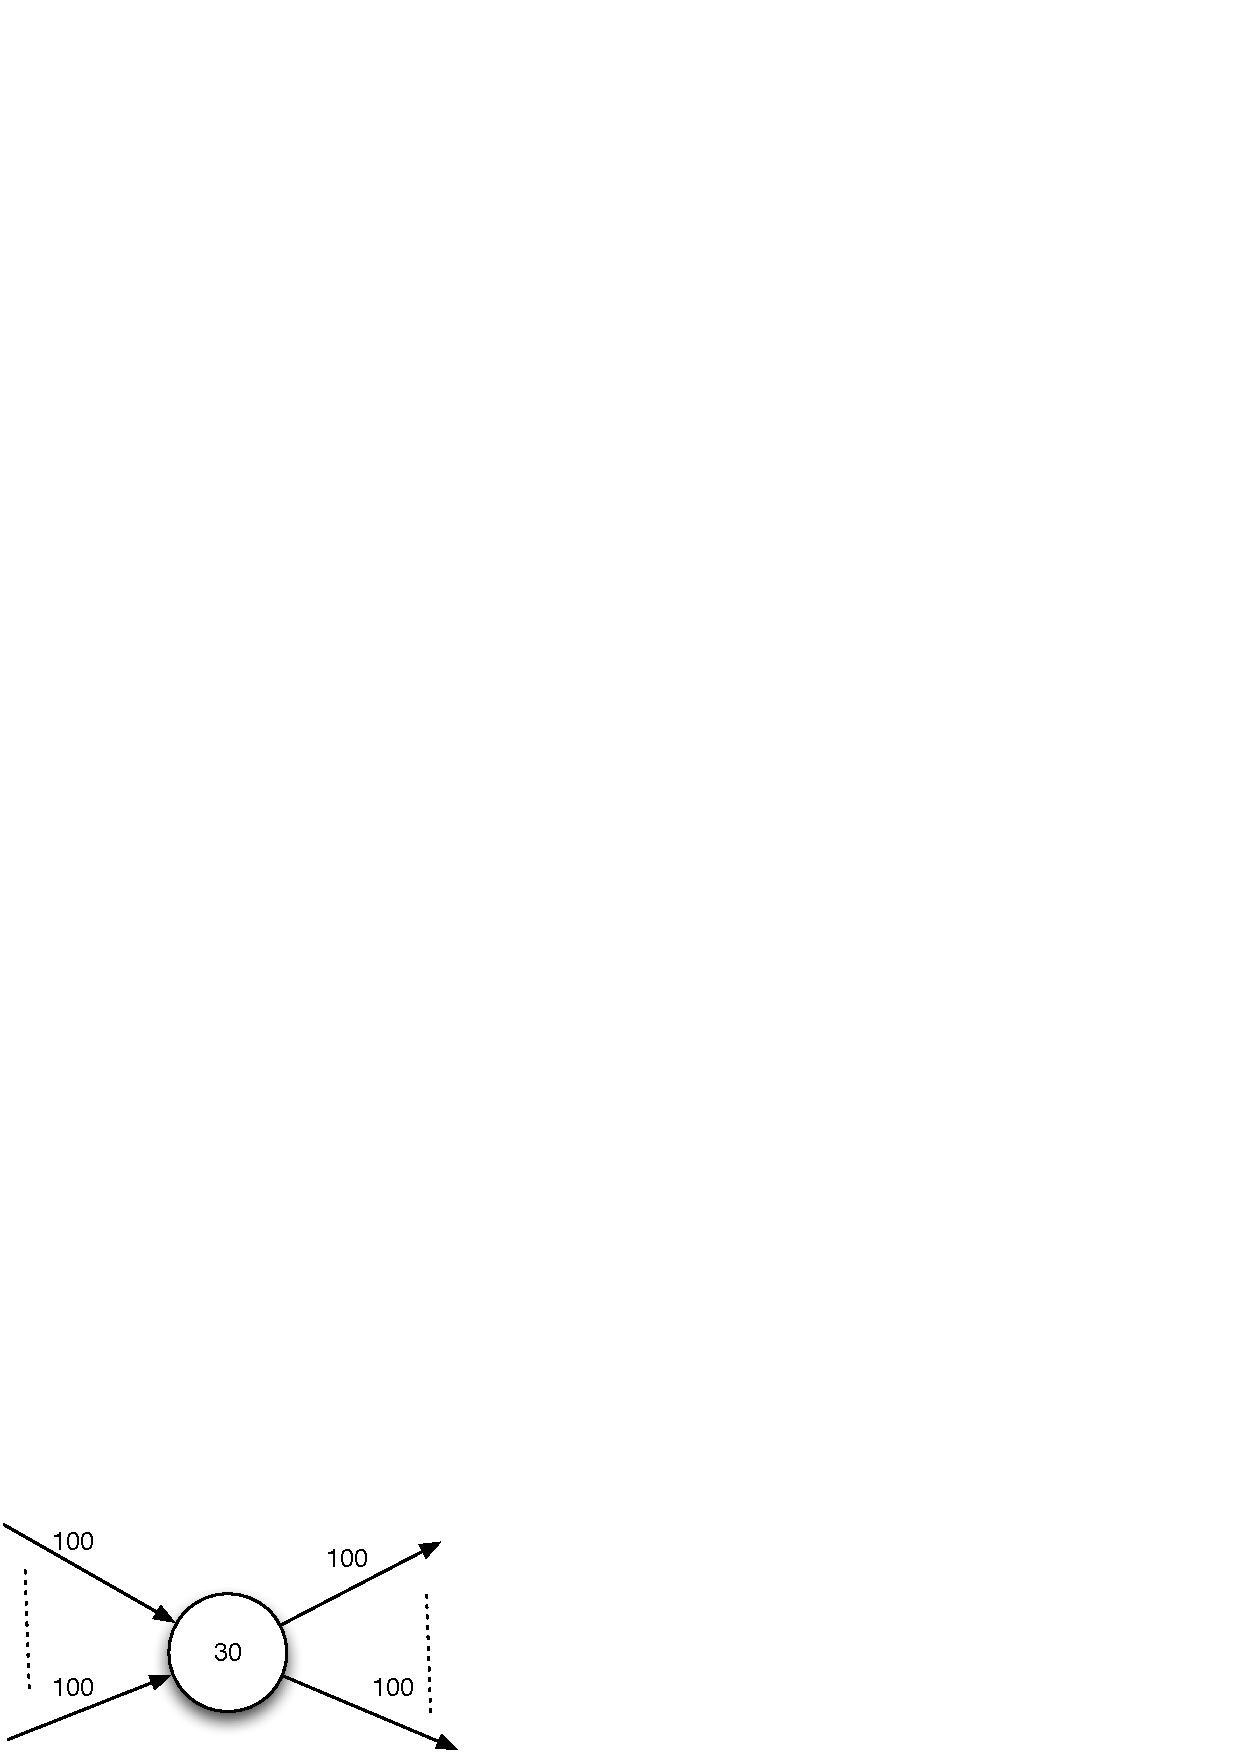
\includegraphics[width=0.4\textwidth]{figures/fig1.pdf}} \quad
    \subfigure[Graph shown in figure \ref{sfig1} transformed so the capacity constraints of the vertices are moved to the edges.]{\label{sfig2}\includegraphics[width=0.5\textwidth]{figures/fig2.pdf}}
}                    
\caption{For each vertex the transformation shown in figure \ref{sfig1} and \ref{sfig2} is performed, yielding a transformed graph, whre the vertices constraints are transformed into edge constraints.}
\label{fig1}
\end{figure}


% section question_2_1 (end)

\section*{Question 2.2} % (fold)
\label{sec:question_2_2}
To accommodate for the capacity constrains on the vertices in \eqref{LP}, we need a constrain on the them.
This can be formulated as the sum of the weights of ingoing edges must not be greater than the capacity of the vertex.

The following constrain should be added to \eqref{LP}
\begin{equation}
	\sum_{e=(u,v)} x_e \leq c_v \qquad \forall v \in V \quad 
\end{equation} 
% section question_2_2 (end)

\section*{Question 2.3} % (fold)
\label{sec:question_2_3}

% section question_2_3 (end)

\section*{Question 2.4} % (fold)
\label{sec:question_2_4}

% section question_2_4 (end)



\section*{Question 3.1} % (fold)
\label{sec:question_3_1}
In the following questions we assume that $G = (V,E)$ is a network, but not a flow network, with capacity constraints on the intersections $V$. Furthermore we assume that $G' = (V',E')$ is a flow network obtained by modifying $G$ as 

A flow in $G$ is a real-valued function $f: V \times V \leftarrow \R$ that satisfies the \emph{capacity constraint} defined as
\begin{equation}
 0 \leq f(u,v) \leq c(u,v) \qquad  \forall u,v \in V
\end{equation}
and the \emph{flow conservation property}
\begin{equation}
\sum_{v \in V} f(v,u) = \sum_{v \in V} f(u,v)  \qquad \forall u \in V \setminus \{s,t\}
\end{equation}
A flow has a value defined by
\begin{equation}
 |f| = \sum_{v \in V} f(s,v) - \sum_{v \in V} f(v,s)
\end{equation}

these properties can be extended so they take intersection-capacities into account by adding a third capacity constraint called the \emph{intersection capacity constraint}. This constraint insures that the maximum flow going into a vertex $u$ is bounded by $c(v)$
\begin{equation}
\sum_{v \in V} f(v,u) \leq c(u) 
\end{equation}
This modification does not affect the flow conservation property or the value, $|f|$, of the flow.


% section question_3_1 (end)

\section*{Question 3.2} % (fold)
\label{sec:question_3_2}
Let $f: V \times V \rightarrow \R$ be a flow in $G$. We can then define the equivalent flow $f': V' \times V' \rightarrow \R$ in $G'$ as
% section question_3_2 (end)

\section*{Question 3.3} % (fold)
\label{sec:question_3_3}
Prove that f' is a flow. That is, given a flow f in G (with capacities on intersections), you convert it to a flow f' in G' (without capacities on intersections) in Question 3.2. The objective of Question 3.3 is then to prove that f' is indeed a flow according to the definitions in the book.
% section question_3_3 (end)

\section*{Question 3.4} % (fold)
\label{sec:question_3_4}

% section question_3_4 (end)


\bibliographystyle{abbrv}
\bibliography{bibliography}

\end{document}                      



